\documentclass{beamer}
\usepackage{graphicx}
\usepackage{graphics}
\usepackage{hyperref}
\usepackage[english]{babel}
\usepackage[T1]{fontenc}
\usepackage[utf8]{inputenc}
\usepackage{xfrac}
\usepackage{ulem}


\mode<presentation>
{
    \usetheme{AMUFree-kk}
    \setbeamercovered{transparent = 28}
}
\title{About distillation, a few words}
\date{2021}
\author{Karol Kaczmarek}
\setbeamertemplate{bibliography item}{[\theenumiv]}


\begin{document}

\begin{frame}
    \titlepage
\end{frame}

\iffalse
\AtBeginSection[]
{
    \begin{frame}
        \frametitle{Outline}
        \tableofcontents[currentsection]
    \end{frame}
}
\fi



% Distillation
\section{Distillation}
\begin{frame}
    \frametitle{Distillation - definition}
    \begin{itemize}
        \item the action of purifying a liquid by a process of heating and cooling
        \item the extraction of the essential meaning or most important aspects of something
    \end{itemize}
    \begin{center}
        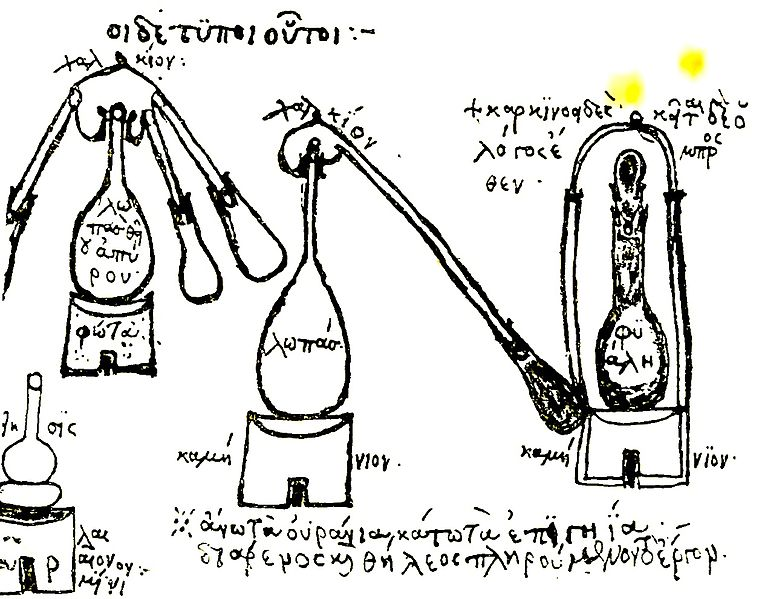
\includegraphics[scale=0.20]{img/zosimos_distillation_equipment.jpg}
        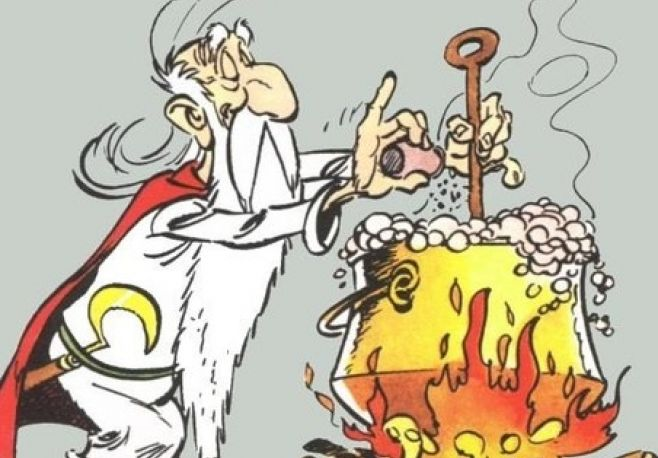
\includegraphics[scale=0.25]{img/kociolek_panoramixa.jpg}
    \end{center}
\end{frame}

\begin{frame}
    \frametitle{Knowledge distillation}
    \begin{itemize}
        \item The \textbf{student} - is trained to reproduce the behavior of a larger model - the \textbf{teacher}
        \item \textbf{Knowledge distillation} (KD) is to train the small \textbf{student} model \textbf{S} on a transfer feature set with soft labels and intermediate representations provided by the large \textbf{teacher} model \textbf{T}.
        \item Knowledge distillation is modeled as minimizing the differences between teacher and student features:
        \begin{itemize}
            \item $ {L}_{\textbf{KD}} = \sum_{e \in D} L({f}^{S}(e), {f}^{T}(e)) $
            \item $ D $ - training data
            \item $ {f}^{S}(\cdot) $ and $ {f}^{T}(\cdot) $ - features of student and teacher models respectively
            \item $ L(\cdot) $ - loss function, often used: \textbf{MSE} - mean squared error or \textbf{KL-divergence} (for probability distribution)
        \end{itemize}
    \end{itemize}
\end{frame}



% DistilBERT
\section{DistilBERT}
\begin{frame}
    \frametitle{DistilBERT \cite{distil_bert}}
    \begin{itemize}
        \item August 2019, HuggingFace -- code available
        \item DistilBERT - pre-trained version of BERT, 40\% smaller, 60\% faster, that retains 97\% of the language understanding capabilities
        \item based on BERT (base)
        \item triple loss combining \textbf{language modeling}, \textbf{distillation} and \textbf{cosine-distance} losses
        \item focus on reducing the number of layers
        \item initialize the student from the teacher by taking one layer out of two (better than random weights initialization)
        \item knowledge distillation during the pre-training phase
    \end{itemize}
\end{frame}

\begin{frame}
    \frametitle{Triple loss functions}
    The final training objective is a linear combination of:
    \begin{itemize}
        \item $ L_{ce} $ - the distillation loss (loss over the soft target probabilities of the teacher, use \textit{softmax-temperature} -- controls the smoothness of the output distribution)
        \item $ L_{mlm} $ - the supervised training loss (the masked language modeling loss)
        \item $ L_{cos} $ - the cosine embedding loss (align the directions of the student and teacher hidden states vectors)
    \end{itemize}
    \begin{center}
        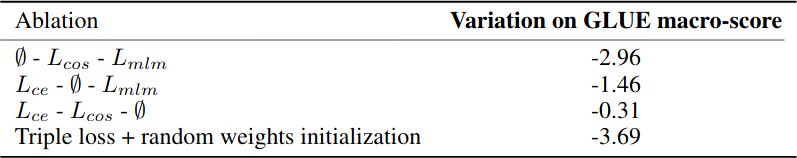
\includegraphics[scale=0.4]{img/distil_bert_ablation.png}
    \end{center}
\end{frame}

\begin{frame}
    \frametitle{GLUE results (dev-set) and inference time}
    \begin{itemize}
      \item GLUE results
      \begin{itemize}
          \item \textbf{BERT}: 12 layers and 768 hidden size
          \item \textbf{DistilBERT}: 6 layers and 768 hidden size
      \end{itemize}
    \end{itemize}
    \begin{center}
        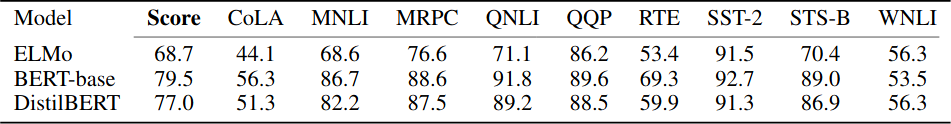
\includegraphics[scale=0.34]{img/distil_bert_glue.png}
    \end{center}
    \begin{itemize}
      \item Inference time (on CPU using a batch size of 1):
    \end{itemize}
    \begin{center}
        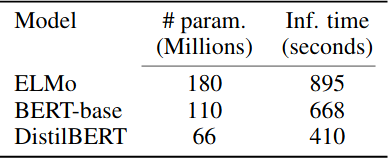
\includegraphics[scale=0.36]{img/distil_bert_inference_time.png}
    \end{center}
\end{frame}

\begin{frame}
    \frametitle{Distillation during fine-tuning}
    \begin{center}
        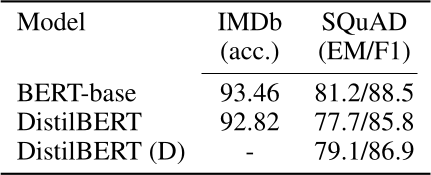
\includegraphics[scale=0.36]{img/distillation_distillation_fine_tune.png}
    \end{center}
\end{frame}



% TinyBERT
\section{TinyBERT}
\begin{frame}
    \frametitle{TinyBERT \cite{tiny_bert}}
    \begin{itemize}
        \item December 2019, Huawei -- code available
        \item TinyBERT - 7,5x smaller, 9,4x faster on inference, that retains 96\% of the language understanding capabilities
        \item based on BERT (base)
        \item design several loss functions to fit different representations from BERT layers
        \item propose a two-stage learning framework including the \textit{general distillation} (distillation + pretraining) and the \textit{task-specific distillation} (distillation + fine-tune + data augmentation)
    \end{itemize}
\end{frame}

\begin{frame}
    \frametitle{Several loss functions}
    Several loss functions are designed to fit different representations from BERT layers:
    \begin{itemize}
        \item the output of the embedding layer
        \item the hidden states and attention matrices derived from the Transformer layer
        \item the logits output by the prediction layer
    \end{itemize}
    \begin{center}
        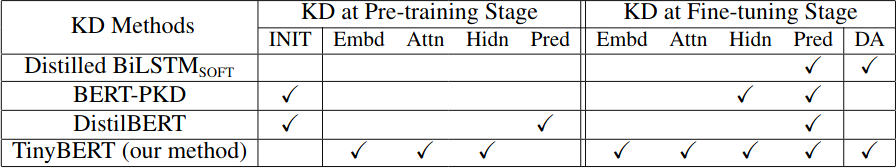
\includegraphics[scale=0.365]{img/tiny_bert_summary.png}
    \end{center}
\end{frame}

\begin{frame}
    \frametitle{Transformer distillation}
    \begin{center}
        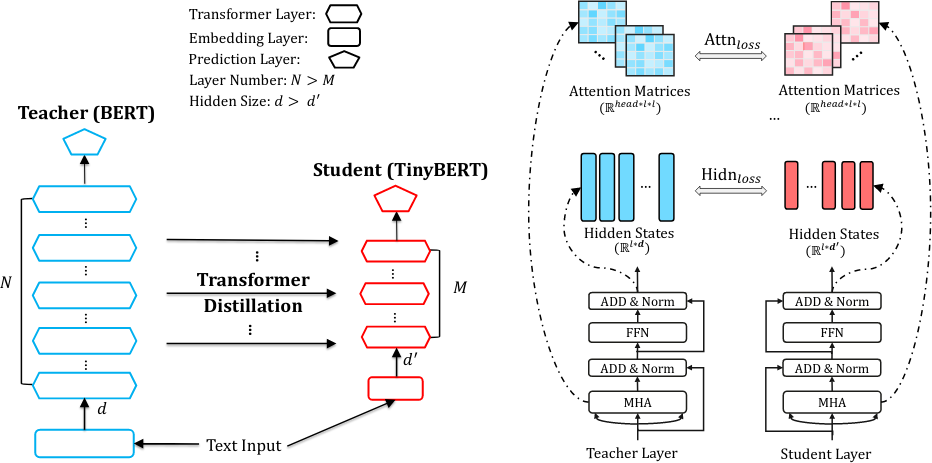
\includegraphics[scale=0.34]{img/tiny_bert_overwiev.png}
    \end{center}
\end{frame}

\begin{frame}
    \frametitle{Transformer distillation}
    \begin{itemize}
        \item Transformer-layer distillation include:
        \begin{itemize}
          \item attention based distillation: $ L_{attn} = \frac{1}{h} \sum_{i = 1}^{h} MSE(A_i^S, A_i^T) \ $
          \item hidden states based distillation: $ L_{hidn} = MSE(H^S W_h, H^T) \ $
        \end{itemize}
        \item embedding-layer distillation: $ L_{embd} = MSE(E^S W_e, E^T) \ $
        \item prediction-layer distillation: soft cross-entropy loss between student and teacher \textbf{logits}
    \end{itemize}
    \tiny Where: $h$ - number of attention heads, $A_i$ - attention matrix (not \textit{softmax} output), $H^{S}$, $H^{T}$ - hidden states (FFN layer), $W_h$ - learnable linear transformation, $E^{S}$, $E^{T}$ - embeddings, $W_e$ - learnable linear transformation
\end{frame}

\begin{frame}
    \frametitle{Learning illustration}
    \begin{center}
        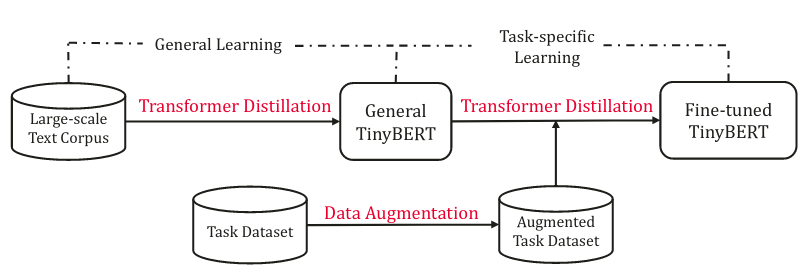
\includegraphics[scale=0.34]{img/tiny_bert_learing.png}
    \end{center}
\end{frame}

\begin{frame}
    \frametitle{GLUE results (test-set) and inference time}
    \begin{itemize}
      \item GLUE results (\textbf{TinyBERT}: 4 layers and 312 hidden size):
    \end{itemize}
    \begin{center}
        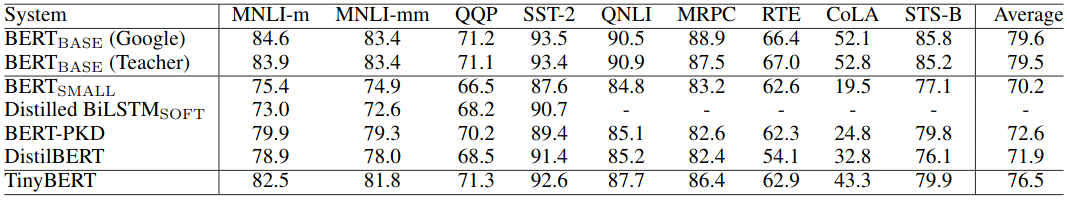
\includegraphics[scale=0.3]{img/tiny_bert_glue.png}
    \end{center}
    \begin{itemize}
      \item Inference time:
    \end{itemize}
    \begin{center}
        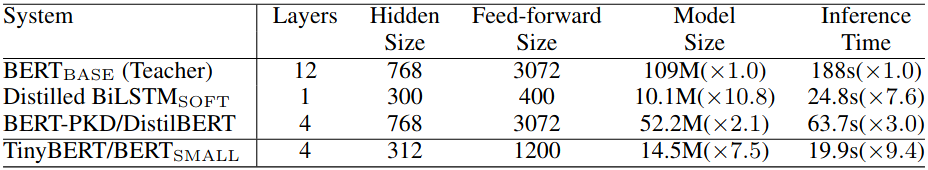
\includegraphics[scale=0.34]{img/tiny_bert_inference_time.png}
    \end{center}
\end{frame}

\begin{frame}
    \frametitle{Ablation studies}
    \begin{itemize}
      \item Two-stage learning (TD - Task-specific Distillation, GD - General Distillation, DA - Data Augmentation)
    \end{itemize}
    \begin{center}
        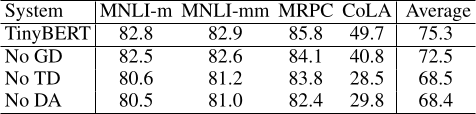
\includegraphics[scale=0.38]{img/tiny_bert_ablation.png}
    \end{center}
    \begin{itemize}
      \item Different distillation objectives
    \end{itemize}
    \begin{center}
        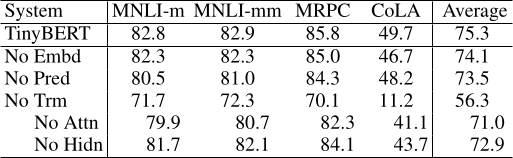
\includegraphics[scale=0.35]{img/tiny_bert_ablation_2.png}
    \end{center}
\end{frame}




% MobileBERT
\section{MobileBERT}
\begin{frame}
    \frametitle{MobileBERT \cite{mobile_bert}}
    \begin{itemize}
        \item April 2020, Google -- code available
        \item MobileBERT - 4,3x smaller, 5,5x faster than BERT (base)
        \item based on BERT (large)
        \item train a specially designed teacher model - an inverted-bottleneck incorporated BERT (large) model
        \item progressive knowledge transfer
        \item task-agnostic lightweight pre-trained model (knowledge transfer in the pre-training stage)
    \end{itemize}
\end{frame}

\begin{frame}
    \frametitle{Inverted-Bottleneck BERT (IB-BERT)}
    \begin{center}
        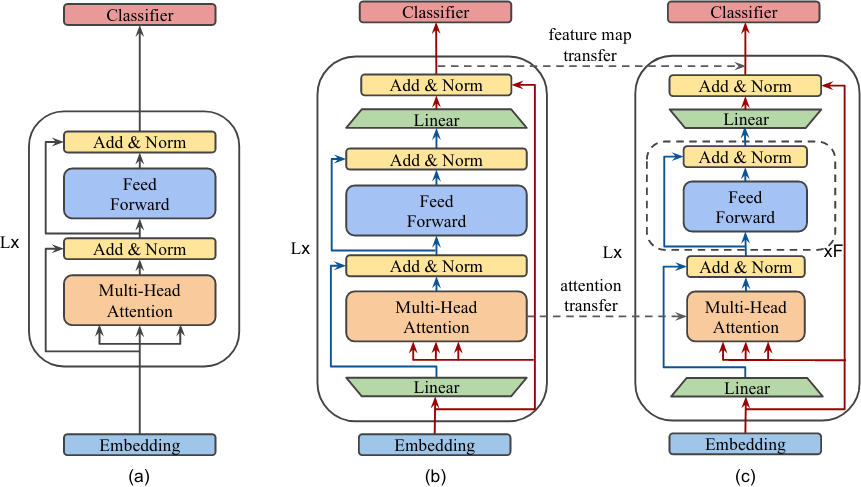
\includegraphics[scale=0.32]{img/mobile_bert_model.png}
    \end{center}
    (a) BERT; (b) IB-BERT; (c) MobileBERT
\end{frame}

\begin{frame}
    \frametitle{Inverted-Bottleneck BERT (IB-BERT)}
    \begin{center}
        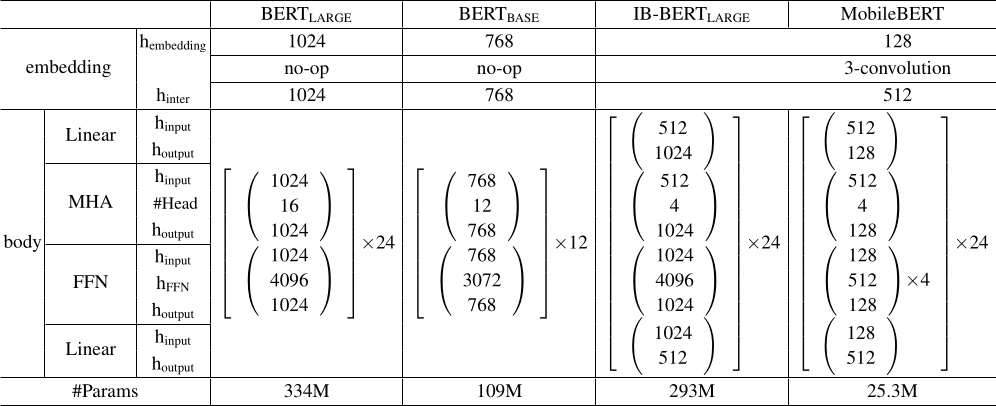
\includegraphics[scale=0.3]{img/mobile_bert_sizes.png}
    \end{center}
\end{frame}

\begin{frame}
    \frametitle{Bottleneck and Inverted-Bottleneck}
    \begin{itemize}
        \item deep as BERT (large), but each building block is made much smaller
        \item the hidden dimension of each building block is only 128 (for MobileBERT)
        \item two linear transformations for each building block to adjust its input and output dimensions to 512
        \item the teacher network (IB-BERT) is just BERT (large) with inverted-bottleneck structures to adjust its feature map size to 512
        \item IB-BERT and MobileBERT have the same feature map size which is 512 (which is used to knowledge transfer)
    \end{itemize}
\end{frame}

\begin{frame}
    \frametitle{Other optimizations}
    \begin{itemize}
        \item stacked Feed-Forward Networks (to avoid more parameters)
        \item remove layer normalization (replace the
layer normalization of a $n$-channel hidden state with an element-wise linear transformation)
        \item use ReLU activation (instead of GELU activation)
        \item reduce the embedding dimension to 128 and apply 1D convolution with kernel size 3 on the raw token embedding to produce a 512 dimensional output
    \end{itemize}
\end{frame}

\begin{frame}
    \frametitle{Training Objectives}
    \begin{itemize}
        \item Feature Map Transfer (FMT) - mean squared error between the feature maps: $ L_{FMT}^l = \frac{1}{TN} \sum_{t=1}^T \sum_{n=1}^N (H_{t,l,n}^{tr} - H_{t,l,n}^{st})^2 $
        \item Attention Transfer (AT) - KL-divergence between the per-head self-attention distributions : $ L_{AT} = \frac{1}{TN} \sum_{t=1}^T \sum_{a=1}^N D_{KL}(attn_{t,l,a}^{tr} - attn_{t,l,a}^{st})^2 $
        \item Pre-training Distillation (PD) - linear combination of the original masked language modeling (MLM) loss, next sentence prediction (NSP) loss, and the new MLM Knowledge Distillation (KD) loss: $ L_{PD} = \alpha L_{MLM} + (1 - \alpha) L_{KD} + L_{NSP} $
    \end{itemize}
    \tiny Where: $l$ - index of layers, $T$ - sequence length, $N$ - feature map size, $H$ - feature map, $A$ - number of attention heads
\end{frame}


\begin{frame}
    \frametitle{Training Strategies}
    \begin{center}
        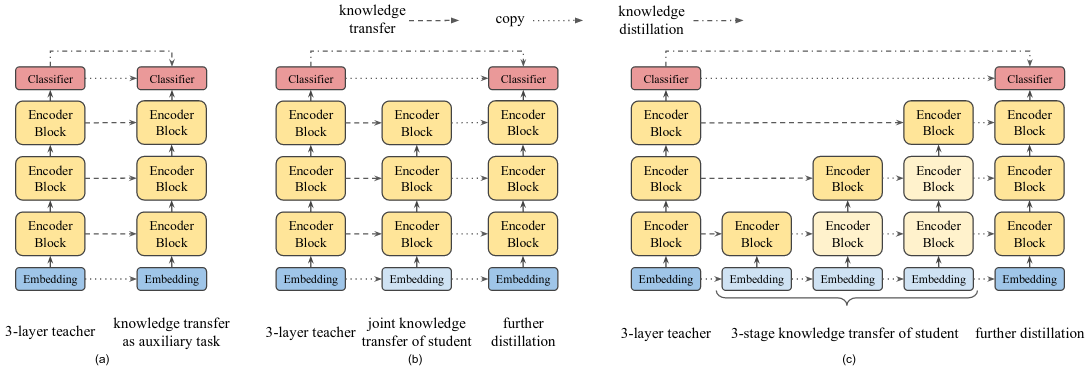
\includegraphics[scale=0.3]{img/mobile_bert_training.png}
    \end{center}
    \tiny(a) Auxiliary Knowledge Transfer; (b) Joint Knowledge Transfer (first train with all layer-wise knowledge transfer losses jointly, and then further train it by pre-training distillation); (c) Progressive Knowledge Transfer (the errors from the lower layers may affect the knowledge transfer in the higher layers)
\end{frame}

\begin{frame}
    \frametitle{GLUE results (test-set)}
    \begin{itemize}
      \item \textbf{MobileBERT}: 24 layers and 128 hidden size
    \end{itemize}
    \begin{center}
        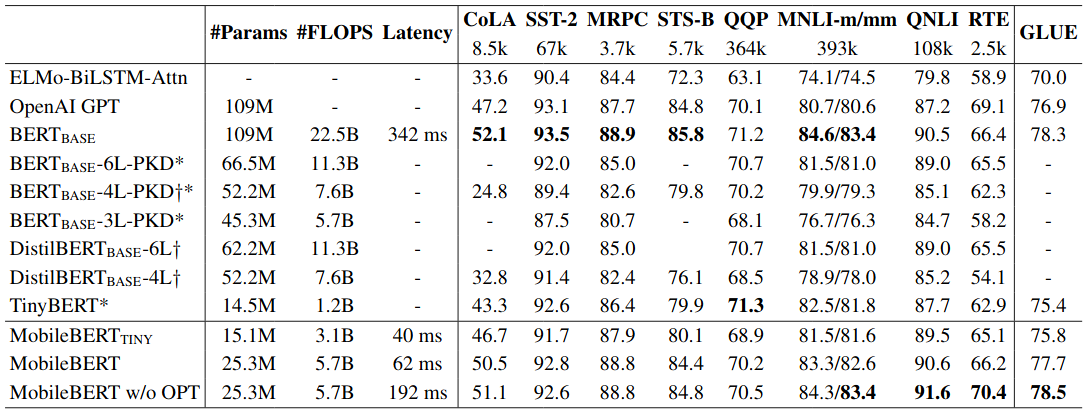
\includegraphics[scale=0.3]{img/mobile_bert_glue.png}
    \end{center}
\end{frame}

\begin{frame}
    \frametitle{The real-world inference latency and the theoretical
computation overhead (FLOPS)}
    \begin{center}
        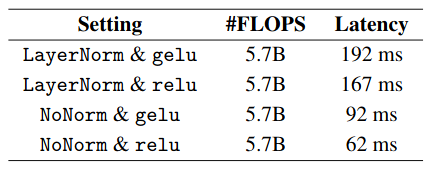
\includegraphics[scale=0.34]{img/mobile_bert_latency.png}
    \end{center}
\end{frame}



% MiniLM
\section{MiniLM}
\begin{frame}
    \frametitle{MiniLM \cite{mini_lm}}
    \begin{itemize}
        \item April/September 2020, Microsoft -- \sout{code available}
        \item based on BERT (base)
        \item Deep Self-Attention Distillation with Teacher Assistant (TA)
        \begin{itemize}
          \item Attention Transfer (Queries-Keys Scaled Dot-Product)
          \item Value-Relation Transfer (Values-Values Scaled Dot-Product)
        \end{itemize}
        \item distillation on the last layer (better than layer-to-layer)
        \item task-agnostic knowledge distillation (pre-training)
    \end{itemize}
\end{frame}

\begin{frame}
    \frametitle{Overview of Deep Self-Attention Distillation}
    \begin{center}
        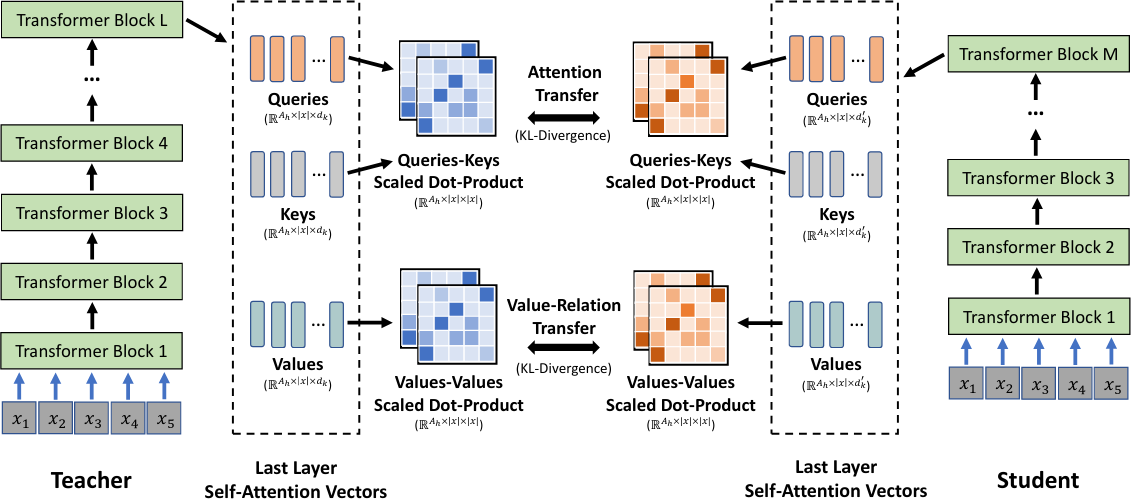
\includegraphics[scale=0.285]{img/mini_lm_distillation.png}
    \end{center}
\end{frame}

\begin{frame}
    \frametitle{Deep Self-Attention Distillation}
    \begin{table}[]
    \begin{tabular}{|c|c|}
    \hline
    Self-Attention & Self-Attention \\
    Distribution Transfer & Value-Relation Transfer \\
    \hline
    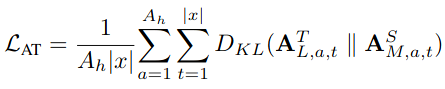
\includegraphics[scale=0.285]{img/mini_lm_self_attention_loss.png} & 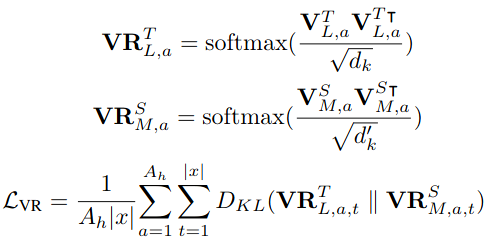
\includegraphics[scale=0.285]{img/mini_lm_values_loss.png} \\
    \hline
    \end{tabular}
    \end{table}
    \tiny Where: $ D_{KL} $ - KL-divergence, $ |x| $ - sequence length,  $ A_h $ - number of attention heads, $L$, $M$ - number of layers for teacher and student

    \normalsize
    \begin{table}[]
    \begin{tabular}{|c|}
    \hline
    Total loss \\
    \hline
    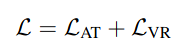
\includegraphics[scale=0.285]{img/mini_lm_total_loss.png} \\
    \hline
    \end{tabular}
    \end{table}
\end{frame}

\begin{frame}
    \frametitle{Teacher Assistant (TA)}
    \begin{itemize}
        \item the teacher model consists of $L$-layer Transformer with $d_h$ hidden size, the student model has $M$-layer Transformer with $d'_h$ hidden size (where $ M \leq \frac{1}{2} L$ and $d'_h \leq \frac{1}{2} d_h$)
        \item Teacher Assistant procedure:
        \begin{enumerate}
           \item distill the \textbf{teacher} into a \textbf{teacher assistant} with $L$-layer Transformer and $ d'_h $ hidden size
           \item distill the \textbf{assistant teacher} into the \textbf{student} with $M$-layer Transformer and $ d'_h $ hidden size
        \end{enumerate}
        \item brings improvements for smaller student models
    \end{itemize}
\end{frame}

\begin{frame}
    \frametitle{Teacher Assistant (TA)}
    \begin{center}
        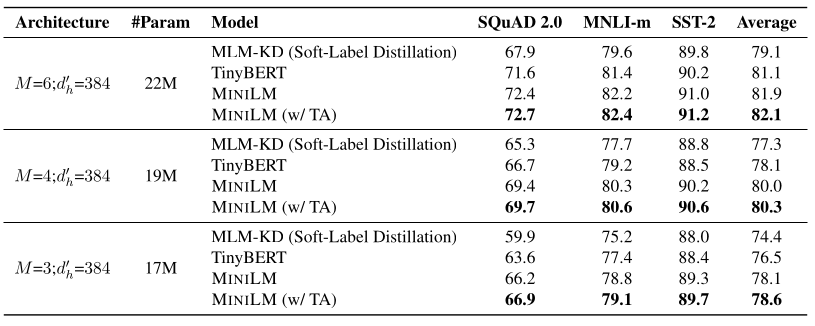
\includegraphics[scale=0.4]{img/minilm_teacher_assistant.png}
    \end{center}
\end{frame}

\begin{frame}
    \frametitle{GLUE results (dev-set) and inference time}
    \begin{itemize}
      \item GLUE results (\textbf{MiniLM}: 6 layers and 768 hidden size):
    \end{itemize}
    \begin{center}
        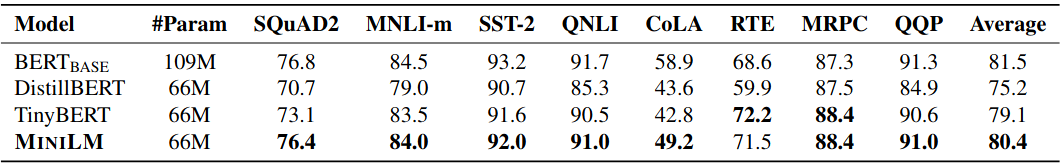
\includegraphics[scale=0.30]{img/mini_lm_glue.png}
    \end{center}
    \begin{itemize}
      \item Inference time (Emd - number of parameters Embedding, Trm - Transformer parameter):
    \end{itemize}
    \begin{center}
        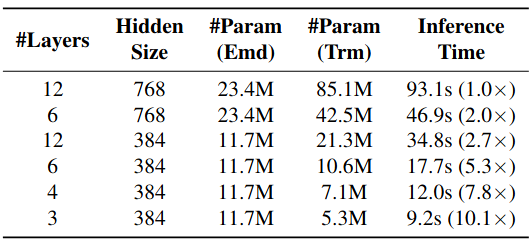
\includegraphics[scale=0.30]{img/mini_lm_inference_time.png}
    \end{center}
\end{frame}



% Distillation approaches
\section{Distillation approaches}
\begin{frame}
    \frametitle{Distillation approaches}
    \begin{center}
        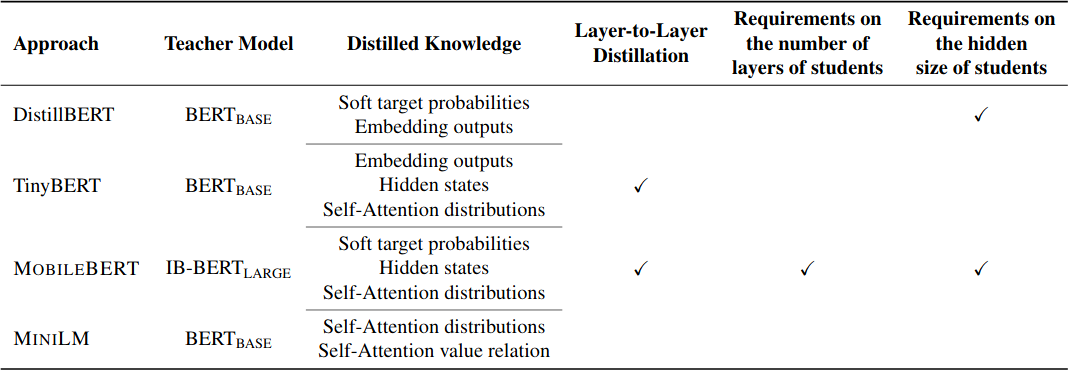
\includegraphics[scale=0.3]{img/distillation_approaches.png}
    \end{center}
\end{frame}



% References
\section{References}
\begin{frame}[allowframebreaks,t]
    \tiny
    \frametitle{References}
    \bibliographystyle{ieeetr}
    \bibliography{model_distillation}
    %\nocite{*}
\end{frame}

\end{document}
